
\documentclass[letter, 9pt, conference]{ieeeconf}

\IEEEoverridecommandlockouts

\overrideIEEEmargins

\usepackage[utf8]{inputenc}
\usepackage[T1]{fontenc}
%\usepackage[top=0.75in, bottom=1in, left=1in, right=1in]{geometry}
\usepackage{xcolor}
\usepackage{graphicx}
\usepackage{hyperref}
\usepackage{minted}

\title{Project report - OVH topology}

\author{Langlois Quentin - 19-28-1700 \and Dardenne Florent - 02-60-1700 \and Iavarone Simon xx-xx-xxxx }


\begin{document}

\maketitle
\thispagestyle{empty}
\pagestyle{empty}


%%%%%%%%%%%%%%%%%%%%%%%%%%%%%%%%%%%%%%%%%%%%%%%%%%%%%%%%%%%%%%%%%%%%%%%%%%%%%%%%
\begin{abstract}

This report will describe our analysis of the European OVH network topology. It will detail different aspects such as oSPF, BGP, security and anycast. At the end, we will present our simulation technique, tests and results. 

\end{abstract}


%%%%%%%%%%%%%%%%%%%%%%%%%%%%%%%%%%%%%%%%%%%%%%%%%%%%%%%%%%%%%%%%%%%%%%%%%%%%%%%%
\section{Introduction}

For this project, we were asked to choose a part of the OVH network, describe and simulate it with the \textbf{ipmininet} library. 

This report will first describe the part of the topology we chose and some information about it such as OSPF and BGP. 

Next, we will present 3 additional aspects such as security, BGP communities and anycast. 

Finally, we will show our simulation methodology, tests and results. 

\section{Description of the topology}

\subsection{Zone description}

We chose the European zone of the topology. This choice was done for 2 reasons : 

\begin{itemize}
    \item There are many redundancies in this part of the network. 
    \item Many external ASes are present at many places which allows us to explore in more details the eBGP mechanism. 
\end{itemize}

\begin{figure}[h!]
    \includegraphics[width=\linewidth]{topo_schema.jpeg}
    \caption{Topology representation}
    \label{fig:topo_schema}
\end{figure}

Legend : 
\begin{itemize}
    \item Boxes represent routers and their color represents their AS (one color per AS). 
    \item Links represent physical links with their associated IGP cost\footnote{See section \ref{sec:ibgp} for more details} (1 by default). 
    \item Circles represent a group of Route-Reflector. 
\end{itemize}



\subsection{OSPF and addressing plan}
\label{sec:ospf}

In order to save a maximum of IP addresses, we chose a \textbf{hierarchical addressing} plan. 

For this purpose, we first assigned a specific subnet for each AS (in /24 for IPv4 and /48 for IPv6). 

Next, we divided the OVH network by region (cities) and gave them a more specific subnet (in /28 for IPv4 and /56 for IPv6). 

The last step was to determine the loopback-address of routers and the address of their interfaces for link addresses. As described in the section \ref{sec:simulation}, we made an incremental address generator for loopback-address and used the same technique for link-addressing. \\
This means we took the first available address (in /32 or /128 for loopback) and assigned it to the router. For the links, we chose the subnet of one of the two routers and generated 2 addresses (in /31 or /127) in order to put the 2 routers in the same subnet. 


\subsection{iBGP configuration}
\label{sec:ibgp}

In order to have a minimal number of iBGP connections, we chose a multi-level Route-Reflector (RR) architecture. 

Furthermore, as shown in Fig. \ref{fig:ibgp_schema}, the iBGP connections follow, in most cases, physical links connections. 

In order to create redundancy, all routers are connected to at least two Route-Reflectors. 

IGP costs allow to avoid diflection also in case of crashes. 

\begin{figure}[h!]
    \includegraphics[width=\linewidth]{ibgp_schema.jpeg}
    \caption{iBGP connections}
    \label{fig:ibgp_schema}
\end{figure}

Description of the RR-levels : 
\begin{itemize}
    \item \textbf{First level} : main level which will dispatch routes to second-level-RR. \\
    We chose \textit{fra-5} and \textit{par-gsw} because they are connected to many other ASes and therefore have a central position and receive many external routes. 
    \item \textbf{Second level} : we splitted the second-level RR in 2 sub-groups:
    \begin{itemize}
        \item At the left of the topology, \textit{milan} and \textit{sbg-g1}, will dispatch routes to this part. 
        \item \textit{ams-5}, \textit{vienne} and \textit{varsovie} which will dispatch routes to the left part of the topology. 
    \end{itemize}
    A fullmesh is done for each subgroups. 
\end{itemize}

\subsection{eBGP configuration}
\label{sec:ebgp}

In order to have a more realistic topology, we had decided to add 1 external AS router for each connection with OVH. Indeed, 1 router connected to Milan, Warsow, Amsterdam,Paris and Frankfurt (for UPC) seemed not realistic at all. 

We chose to make \textbf{client-provider sessions} (where OVH is the provider) as we considered OVH as a transit network. 

\subsection{Topology summary}
\label{sec:summary}

As described in the \ref{sec:simulation} section, we also added methods to print statistics on the topology. Here is a screen of the result. 

\begin{figure}[h!]
    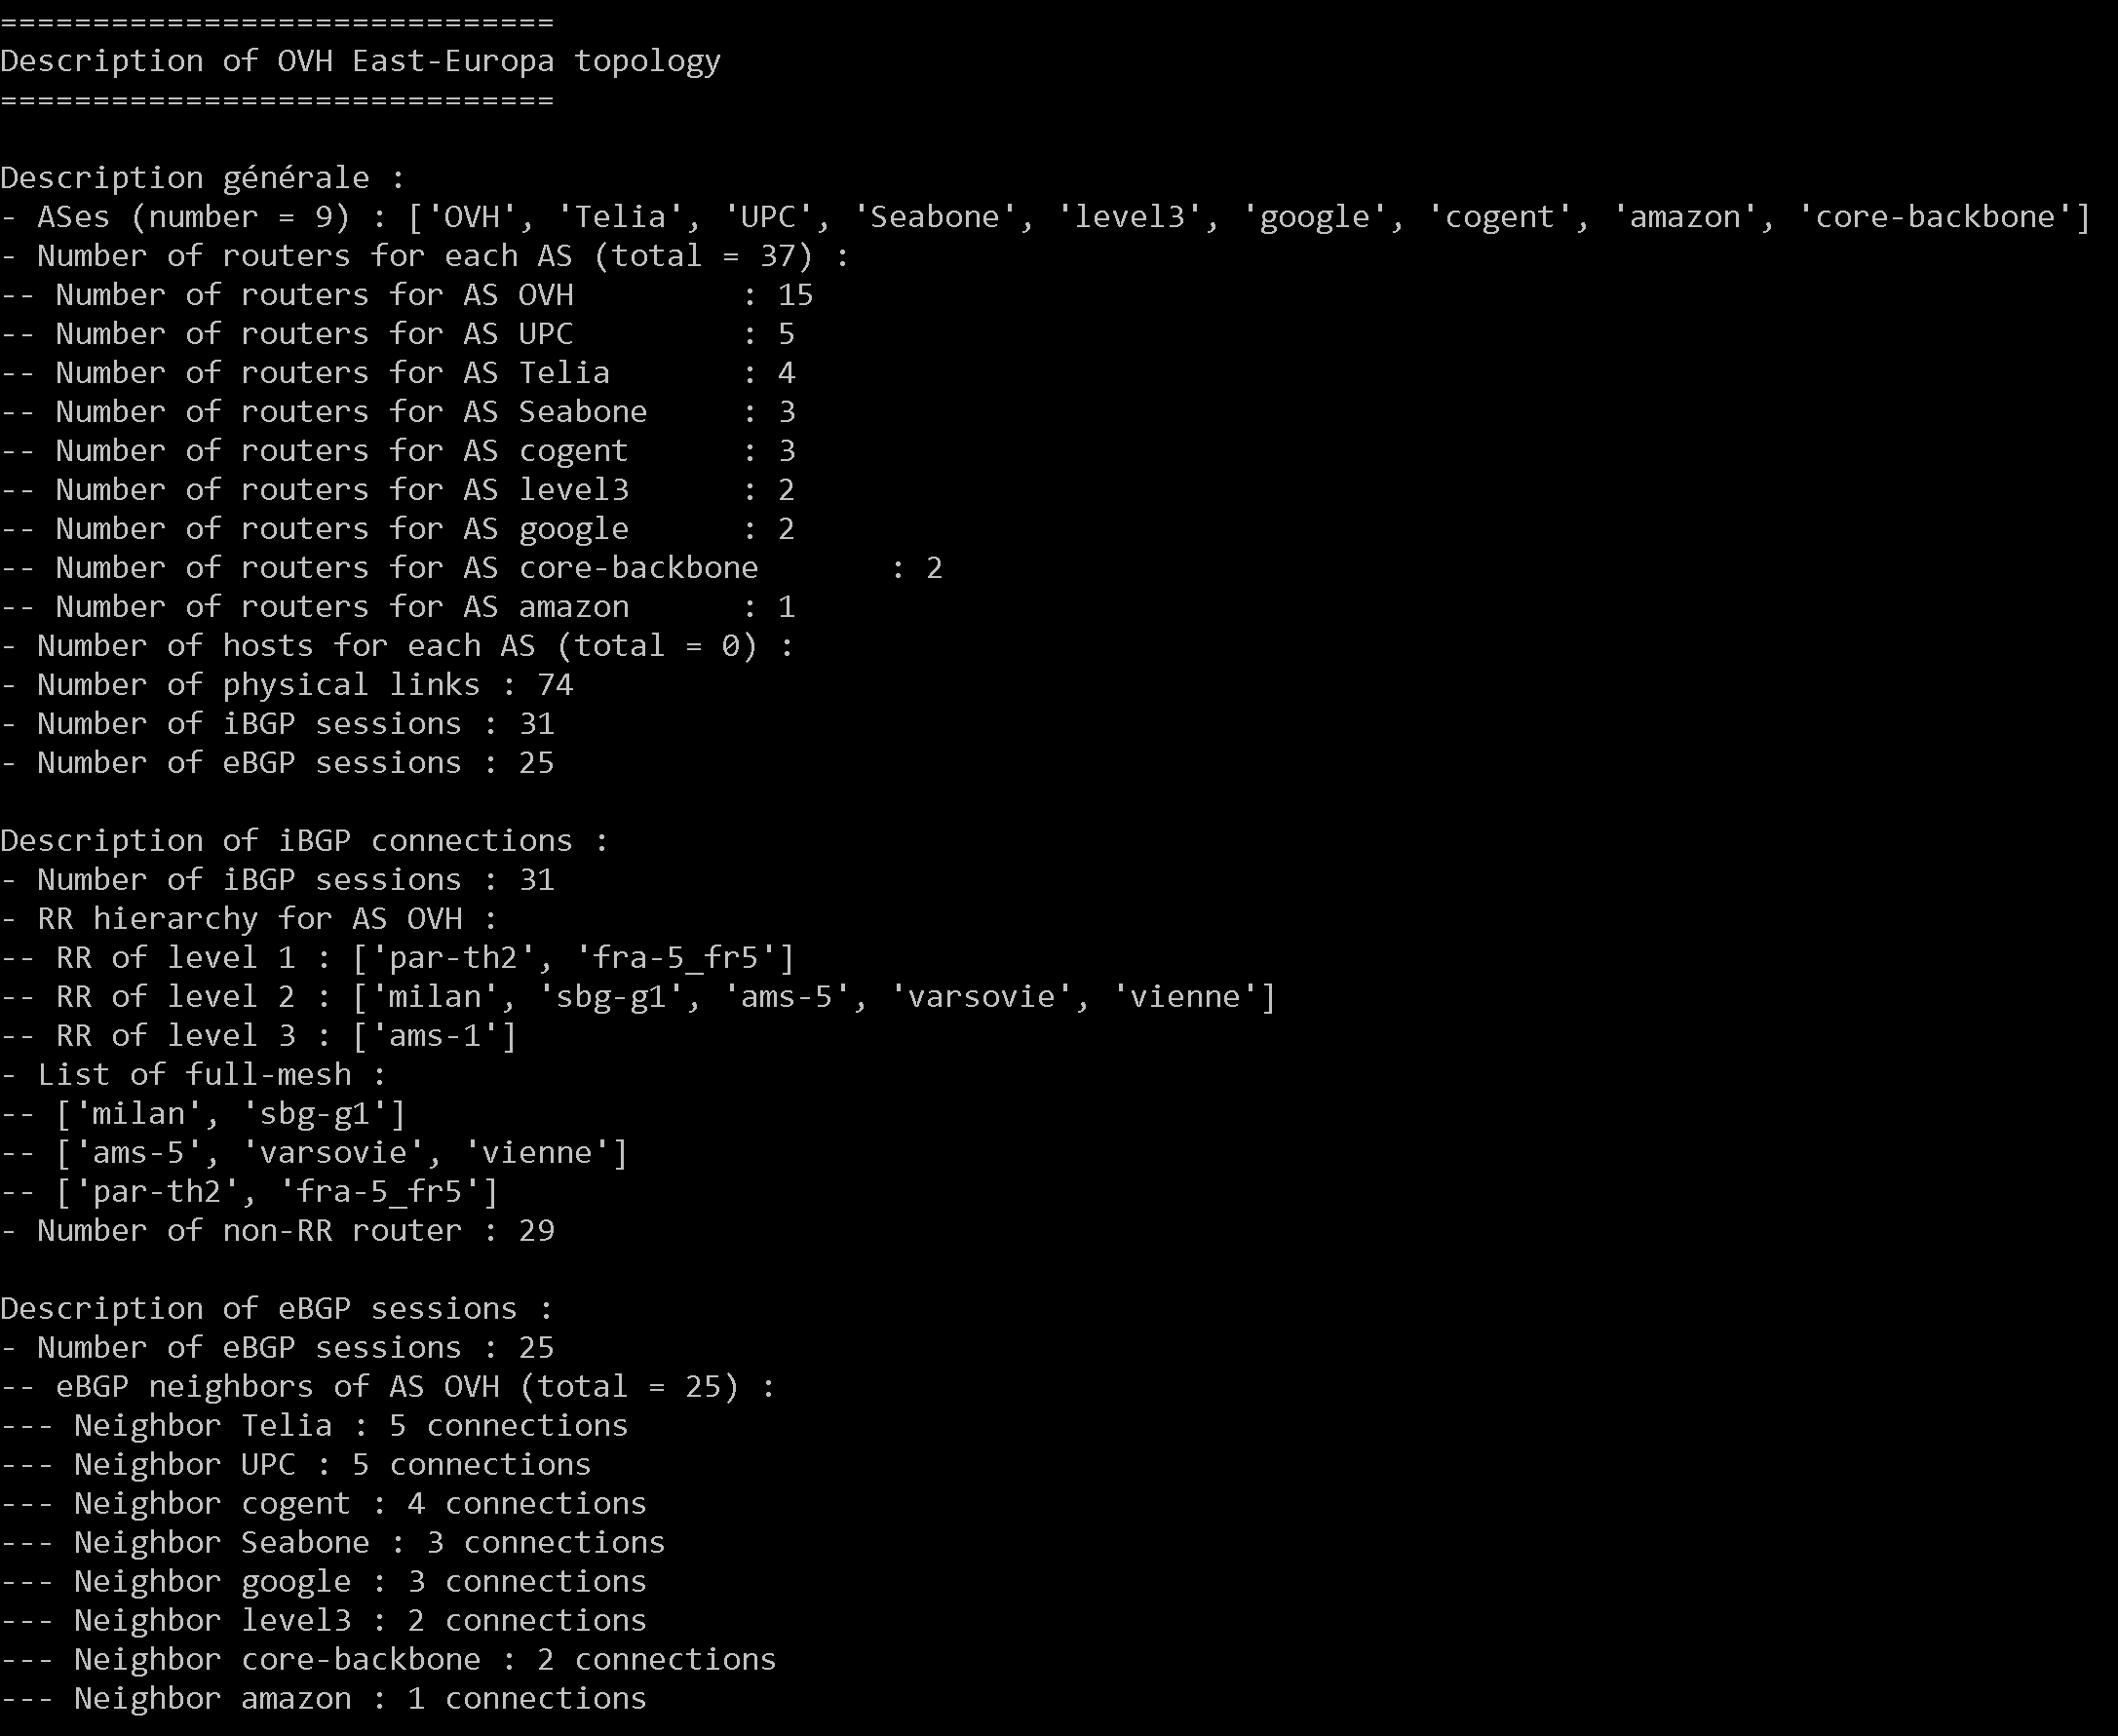
\includegraphics[width=\linewidth]{topo_summary.PNG}
    \caption{Information about the topology}
    \label{fig:topo_summary}
\end{figure}


\section{Security}
\label{sec:security}


\section{BGP communities}
\label{sec:communities}


\section{Anycast}
\label{sec:anycast}

\subsection{Anycast techniques}

Anycast is the ability to have multiple \textbf{servers} with the sime IP address in a network and join the nearest from its position. 

There are many possible utilization for this feature such as DNS servers, data-centers, ... 

In order to configure anycast, there are 3 main ways : 
\begin{itemize}
    \item \textbf{DNS zones} : groups some servers under a unique domain name. 
    \item \textbf{OSPF} : advertise multiple times the same IP address over OSPF. 
    \item \textbf{BGP} : advertise multiple times the same IP address over BGP. 
\end{itemize}

\subsection{Anycast in our topology}

For this project, we chose the third solution : anycast over BGP. \\
Here are some reasons : 
\begin{itemize}
    \item The implementation is pretty easy. 
    \item The BGP decision process allows to advertise the route to thenearest server. 
    \item The convergence in case of failure is relatively fast. 
    \item It allows to use BGP properties such as communities to make traffic engineering. 
    \item It allows to better secure the server's behaviour compared to the OSPF technique. 
\end{itemize}

\subsection{Anycast in our simulation}

More details about the simulation are given in its appropriate session but here, we will just show the anycast aspect of it. 

As we chose the BGP method to implement anycast, the simulation was easy to implement because BGP is well supported by the ipmininet library. 

However, the BGP daemon is not supported by the \textbf{Host} class and we therefore chose to use the \textbf{Router} class to represent anycast servers. 

To specify their common anycast IP address, we just specify it as their loopback-address. 

In order to advertise this anycast address to other AS, we had to connect these anycast servers to a Route-Reflector. To simplify the simulation, we added a new level of Route-Reflector responsible to advertise anycast server's routes\footnote{if their neighbor router was already a RR, we just added the anycast server to its clients.}. 

\section{Simulation}
\label{sec:simulation}

\subsection{JSON representation}
\label{sec:json}

For the project, we had chosen to create an automatized construction of the topology based on a structured representation of it. One of the easiest and most common way to structure data is the \textbf{JSON} format. 

Here is a brief overview of our formatted OVH topology and its different configuration fields :

\begin{minted}{python}
{
# subnets to infer loopback and links addresses
  "subnets" : {
    "net_ovh" : { # Main OVH subnet in /24 and / 48
      "ipv6" : "beaf:cafe:babe:/48",
      "ipv4" : "204.32.46./24"
    },
    "net_mil" : { # Specific subnet in /28 and /56. 
      # Adresses are structured with the 
      # 'net_ovh' field. It will be replaced
      # by the corresponding address of this subnet
      "ipv6" : "{net_ovh}0500::/56",
      "ipv4" : "{net_ovh}112/28",
      "nodes" : ["milan"]
    },
    # ... other subnets for the cities
    "net_upc" : { # Example of subnet for another AS. 
      "ipv6" : "beaf:cafe:bab1::/48",
      "ipv4" : "204.32.48.0/24",
      "nodes" : ["upc_var", "upc_vie", ...]
    },
    # ... other subnets for ASes
  },
  "AS" : {    # ASes in the topology
    "OVH" : { # Our main AS. 
      # Routers in the AS with their configuration. 
      "routers" : {
        # As milan has a 'clients' field, it is considered as a RR. 
        "milan" : { # Name of the router : milan
          # Peers, clients and level for the RR
          # Note : if level is not specified, default = 1
          # 'peers' should only be specified for level > 1
          "clients" : ["zurich", "sbg-g2"],
          "peers" : ["sbg-g1"],
          "niveau" : 2
        },
        "zurich": {}, # Simple router without config
        # ... other routers
      },
      # Default config for all routers of this AS
      "rconfig" : {
        "daemons" : {   # Default daemons
          "ospf": {}, "ospf6":{}, # Daemons without config
          "bgp": {    # Config for the BGP daemon
            "communities": {    # Communities to add
              "set_local_pref": { # Conditionned Local-pref
                "16276:120": 120
              }
            }
          }
        }
      },
      "anycast" : [ # Anycast servers in this AS
        {
          "addresses" : { # Anycast addresses
            "ipv4": "10.10.10.10/32", 
            "ipv6": "10::10/128"
          },
          # Nodes to which connect an anycast server
          "nodes" : ["milan", "varsovie", "ams-1"]
        }
      ]
      # the field 'hosts' can also be added 
      # to specify hosts in the AS
      # In our case, we did not have any hosts 
      # so this field is not present. 
      # However, for our tests, we added many 
      # fictitious hosts automatically
    },
    "Telia" : {
      "routers" : { ... },
      "rconfig" : {
        # Daemons are specified as a list (no config)
        "daemons" : ["ospf", "ospf6", "bgp"]
      },
      # Automatically create a fullmesh of links
      # between all routers of the AS
      "linked" : true
      # Automatically create a iBGP fullmesh
      "bgp_fullmesh" : true
    },
    # ... other AS configuration
  },
  "links" : {   # Physical links
    "milan"    : [  # Node and its neighbors
      "zurich",   # Link without config
      # Link with specified IGP metric
      ["sbg-g1", {"igp_metric": 4}],
      ["sbg-g2", {"igp_metric": 4}]
    ],
    # ... Other links
    # Example of a link between routers from 2 different AS. 
    # The code will automatically create an eBGP connection between them
    "amazon_par"  : ["par-th2"]
  }
}

\end{minted}


\subsection{Topology generation}

In this section, we will describe briefly the main aspects of the topology generation that are useful to understand our tests. 

Indeed, a a more detailed description of each part of the construction (AS, routers, links and subnets) can be found on our code. 

\subsubsection{IP address generator}

In order to generate easily IP addresses, we created an IP address generator based on a specific subnet. This generator is used in 2 features : loopback-address and link-address generation. 

For the loopback-address part, the target is to create a /32 (or /128) address based on the router's subnet. As shown in the section \ref{sec:json}, we can easily get the subnet of a specific router. \\
After the identification, we get the number of already created address for this subnet, add 1 to the last byte and get the new address. 

For the links-addresses, the difficulty was to create a /31 (or /127) address so we had to get the right subnet (and not add 1 like for loopback address). \\
To solve it, we compute the next multiple of 2 ($ 2^(32 - 31) $) for the last byte and it gives us the first address of the subnet. We then compute the second address by adding 1 to the last byte. \\
\textbf{Note} : to select the subnet for the link, we take the subnet of the "main"\footnote{the main note is the key in our json-format of links. The values are its neighbors} node of the link.

\subsubsection{Hosts generator}

In order to make tests on our topology (ping, traceroute) we also provide a tool to add fictitious hosts to AS\footnote{A more detailed description of the different features of this tool can be found in the documentation of our \textit{JSONTopo class}}.

As a basic usage, we simply added 1 host for each router of each AS. With this technique, we were able to test connections between all parts of our topology. 

\subsection{Tests}

For our tests, we used the \textbf{Mininet command-line} to execute commands on our routers. Here is a brief overview of commands used to test differents aspects : 

\begin{itemize}
    \item \textbf{OSPF and BGP} : as shown in the previous section, we added many many fictitious hosts in our topology. This allows us to test the connectivity between all pairs of routers with the \textbf{ping6all} command. 
    
    \item \textbf{Security} : 
    
    \item \textbf{BGP communities} : 
    
    \item \textbf{Anycast} : in order to test Anycast, we added 3 anycast-servers in different places (cf section \ref{sec:json}, anycast entry). Next, we used the traceroute command from differents hosts (inside / outside our AS) to the anycast address and see which server has been reached. 
\end{itemize}

\subsection{Results}

\paragraph{OSPF and BGP results :} with the \textbf{ping6all} command, all hosts tried to contact each other hosts so that we could check if all prts of our network is reachable by all other parts. The result of the command showed a 0\% packet drop : it means that all routes are well distributed and reachable in the whole topology. 

\paragraph{Security :}

\paragraph{BGP communities :}

\paragraph{Anycast :} as mentionned in the section \ref{sec:json}, we created 3 anycast servers in milan, Warsow and Amsterdam. We then used our fictitious hosts in different regions to see which router is reached and here is the results : 

\begin{figure}[h!]
    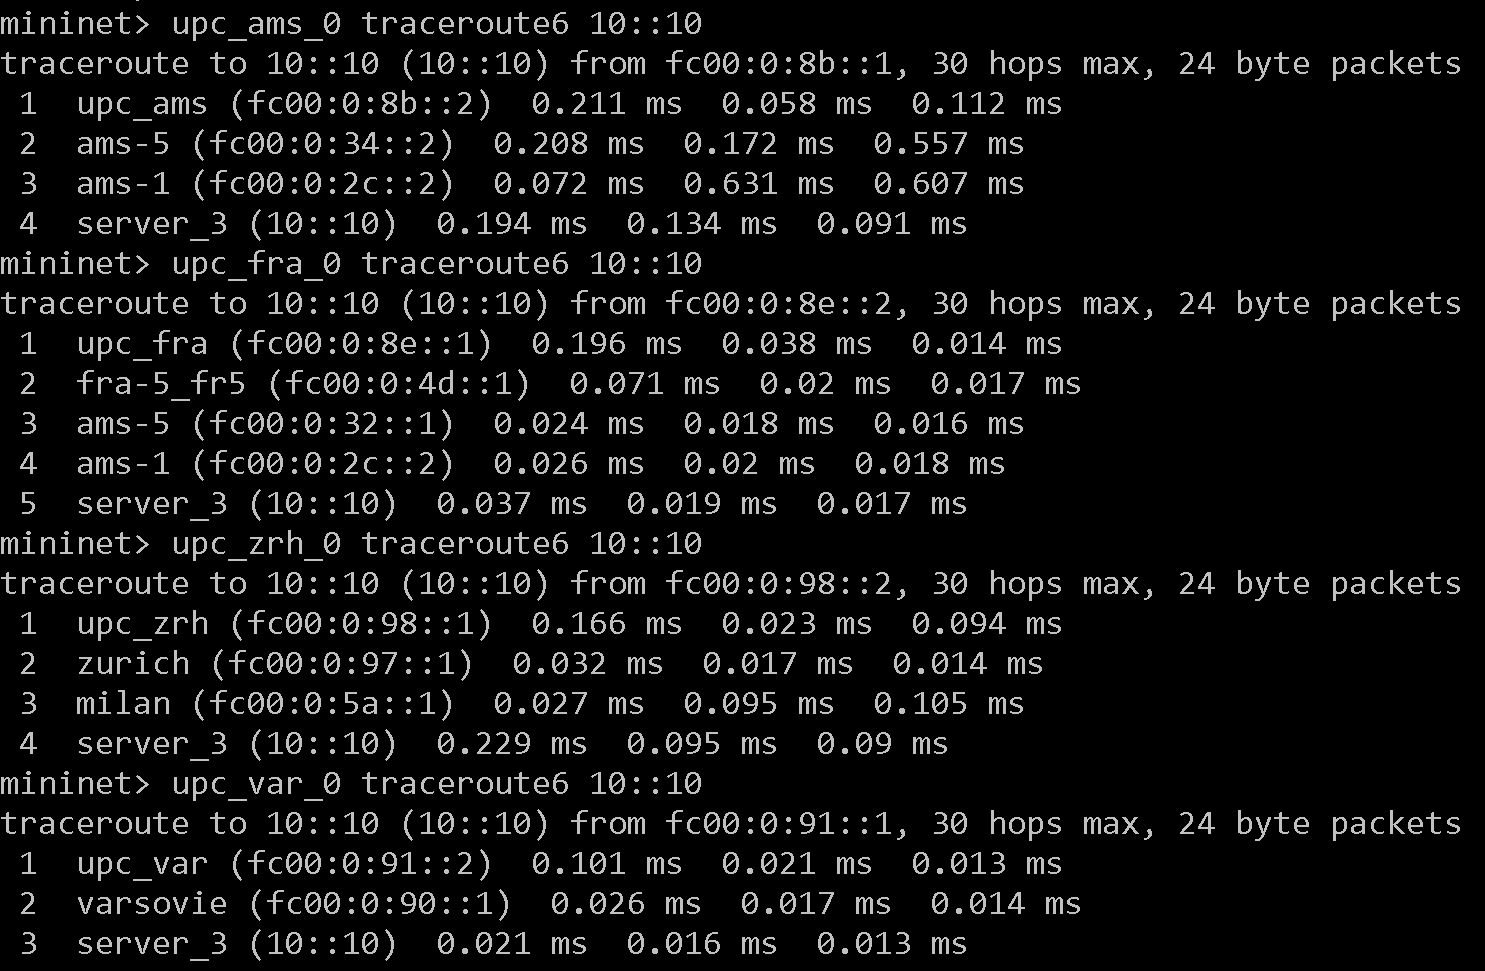
\includegraphics[width=\linewidth]{anycast_test.PNG}
    \caption{Anycast testing with traceroute}
    \label{fig:anycast_test}
\end{figure}

As shown in the figure, all hosts contacted the nearest anycast server\footnote{The server names are not always correct thanks to the ipmininet reverse DNS but we can identify the right server by the last router reached} as we expected. 

\section{Conclusion}


\addtolength{\textheight}{-10cm}   % This command serves to balance the column lengths
                                  % on the last page of the document manually. It shortens
                                  % the textheight of the last page by a suitable amount.
                                  % This command does not take effect until the next page
                                  % so it should come on the page before the last. Make
                                  % sure that you do not shorten the textheight too much.

%%%%%%%%%%%%%%%%%%%%%%%%%%%%%%%%%%%%%%%%%%%%%%%%%%%%%%%%%%%%%%%%%%%%%%%%%%%%%%%%



%%%%%%%%%%%%%%%%%%%%%%%%%%%%%%%%%%%%%%%%%%%%%%%%%%%%%%%%%%%%%%%%%%%%%%%%%%%%%%%%



\begin{thebibliography}{99}

\bibitem{c1} Keynote iPad application : for schemas. 
\bibitem{c2} ipmininet : for the simulation
\bibitem{c3} 
\bibitem{c4} 
\bibitem{c5} 
\bibitem{c6} 
\bibitem{c7} 
\bibitem{c8} 
\bibitem{c9} 
\bibitem{c10} 
\bibitem{c11} 
\bibitem{c12} 

\bibitem{c13} https://docs.umbrella.com/deployment-umbrella/docs/configure-anycast
\bibitem{c14} https://citeseerx.ist.psu.edu/viewdoc/download?doi=10.1.1.116.6367&rep=rep1&type=pdf

\bibitem{c15} http://routedo.com/posts/frr-ospf
\bibitem{c16} https://documentation.nokia.com/html/0\_add-h-f/93-0267-HTML/7X50\_Advanced\_Configuration\_Guide/BGP\_anycast.pdf
\bibitem{c17} https://serverius.net/bgp-anycast-dual-datacenter-using-1-ip-multiple-locations/
\bibitem{c18} https://ipmininet.readthedocs.io/en/latest/daemons.html#named


\end{thebibliography}


\end{document}
